\documentclass[tikz]{standalone}

\usepackage{pgfplots}
\usepackage{amsmath,amssymb,amsfonts}

\pgfplotsset{compat=newest}
\pgfplotsset{every axis/.append style={
                    axis x line=middle,
                    axis y line=middle,
                    axis line style={<->},
                    xlabel={$x$},
                    ylabel={$y$},
                    label style={font=\scriptsize},
                    xticklabel style={
                                    font=\tiny,
                                    yshift=2pt
                                },
                                yticklabel style={
                                    font=\tiny,
                                    xshift=3pt
                                },
                    unit vector ratio*=1 1 1,
   					xlabel style={at={(ticklabel* cs:1)},anchor=west},
   					ylabel style={at={(ticklabel* cs:1)},anchor=south}
                    }}
\begin{document}

  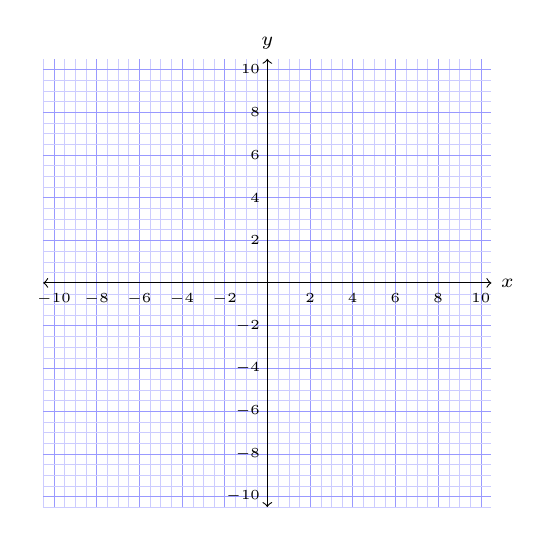
\begin{tikzpicture}

   \begin{axis}[
	 name = graph1,
     ytick distance = 2,
     xtick distance = 2,
     ymin=-10.5, ymax=10.5,
     xmin=-10.5, xmax=10.5,
     grid=both,
     grid style={line width=.05pt,draw=blue!20},
     major grid style={line width=.15pt,draw=blue!40},
     minor tick num=3,
     tick style={draw=none},
   ]

   \end{axis}

  \end{tikzpicture}

\end{document}